% This contents of this file will be inserted into the _Solutions version of the
% output tex document.  Here's an example:

% If assignment with subquestion (1.a) requires a written response, you will
% find the following flag within this document: <SCPD_SUBMISSION_TAG>_1a
% In this example, you would insert the LaTeX for your solution to (1.a) between
% the <SCPD_SUBMISSION_TAG>_1a flags.  If you also constrain your answer between the
% START_CODE_HERE and END_CODE_HERE flags, your LaTeX will be styled as a
% solution within the final document.

% Please do not use the '<SCPD_SUBMISSION_TAG>' character anywhere within your code.  As expected,
% that will confuse the regular expressions we use to identify your solution.
\def\assignmentnum{1 }
\def\assignmenttitle{XCS236 Problem Set \assignmentnum}

\documentclass{article}
\usepackage[top = 1.0in]{geometry}

\usepackage{graphicx}

\usepackage[utf8]{inputenc}
\usepackage{listings}
\usepackage[dvipsnames]{xcolor}
\usepackage{bm}
\usepackage{algorithm}
\usepackage{algpseudocode}
\usepackage{framed}

\definecolor{codegreen}{rgb}{0,0.6,0}
\definecolor{codegray}{rgb}{0.5,0.5,0.5}
\definecolor{codepurple}{rgb}{0.58,0,0.82}
\definecolor{backcolour}{rgb}{0.95,0.95,0.92}

\lstdefinestyle{mystyle}{
    backgroundcolor=\color{backcolour},   
    commentstyle=\color{codegreen},
    keywordstyle=\color{magenta},
    stringstyle=\color{codepurple},
    basicstyle=\ttfamily\footnotesize,
    breakatwhitespace=false,         
    breaklines=true,                 
    captionpos=b,                    
    keepspaces=true,                 
    numbersep=5pt,                  
    showspaces=false,                
    showstringspaces=false,
    showtabs=false,                  
    tabsize=2
}

\lstset{style=mystyle}

\newcommand{\di}{{d}}
\newcommand{\nexp}{{n}}
\newcommand{\nf}{{p}}
\newcommand{\vcd}{{\textbf{D}}}
\newcommand{\Int}{\mathbb{Z}}
\newcommand\bb{\ensuremath{\mathbf{b}}}
\newcommand\bs{\ensuremath{\mathbf{s}}}
\newcommand\bp{\ensuremath{\mathbf{p}}}
\newcommand{\relu} { \operatorname{ReLU} }
\newcommand{\smx} { \operatorname{softmax} }
\newcommand\bx{\ensuremath{\mathbf{x}}}
\newcommand\bz{\ensuremath{\mathbf{z}}}
\newcommand\bh{\ensuremath{\mathbf{h}}}
\newcommand\bc{\ensuremath{\mathbf{c}}}
\newcommand\bW{\ensuremath{\mathbf{W}}}
\newcommand\by{\ensuremath{\mathbf{y}}}
\newcommand\bo{\ensuremath{\mathbf{o}}}
\newcommand\be{\ensuremath{\mathbf{e}}}
\newcommand\ba{\ensuremath{\mathbf{a}}}
\newcommand\bu{\ensuremath{\mathbf{u}}}
\newcommand\bv{\ensuremath{\mathbf{v}}}
\newcommand\bP{\ensuremath{\mathbf{P}}}
\newcommand\bg{\ensuremath{\mathbf{g}}}
\newcommand\bX{\ensuremath{\mathbf{X}}}
% real numbers R symbol
\newcommand{\Real}{\mathbb{R}}

% encoder hidden
\newcommand{\henc}{\bh^{\text{enc}}}
\newcommand{\hencfw}[1]{\overrightarrow{\henc_{#1}}}
\newcommand{\hencbw}[1]{\overleftarrow{\henc_{#1}}}

% encoder cell
\newcommand{\cenc}{\bc^{\text{enc}}}
\newcommand{\cencfw}[1]{\overrightarrow{\cenc_{#1}}}
\newcommand{\cencbw}[1]{\overleftarrow{\cenc_{#1}}}

% decoder hidden
\newcommand{\hdec}{\bh^{\text{dec}}}

% decoder cell
\newcommand{\cdec}{\bc^{\text{dec}}}

\usepackage[hyperfootnotes=false]{hyperref}
\hypersetup{
  colorlinks=true,
  linkcolor = blue,
  urlcolor  = blue,
  citecolor = blue,
  anchorcolor = blue,
  pdfborderstyle={/S/U/W 1}
}
\usepackage{nccmath}
\usepackage{mathtools}
\usepackage{graphicx,caption}
\usepackage[shortlabels]{enumitem}
\usepackage{epstopdf,subcaption}
\usepackage{psfrag}
\usepackage{amsmath,amssymb,epsf}
\usepackage{verbatim}
\usepackage{cancel}
\usepackage{color,soul}
\usepackage{bbm}
\usepackage{listings}
\usepackage{setspace}
\usepackage{float}
\definecolor{Code}{rgb}{0,0,0}
\definecolor{Decorators}{rgb}{0.5,0.5,0.5}
\definecolor{Numbers}{rgb}{0.5,0,0}
\definecolor{MatchingBrackets}{rgb}{0.25,0.5,0.5}
\definecolor{Keywords}{rgb}{0,0,1}
\definecolor{self}{rgb}{0,0,0}
\definecolor{Strings}{rgb}{0,0.63,0}
\definecolor{Comments}{rgb}{0,0.63,1}
\definecolor{Backquotes}{rgb}{0,0,0}
\definecolor{Classname}{rgb}{0,0,0}
\definecolor{FunctionName}{rgb}{0,0,0}
\definecolor{Operators}{rgb}{0,0,0}
\definecolor{Background}{rgb}{0.98,0.98,0.98}
\lstdefinelanguage{Python}{
    numbers=left,
    numberstyle=\footnotesize,
    numbersep=1em,
    xleftmargin=1em,
    framextopmargin=2em,
    framexbottommargin=2em,
    showspaces=false,
    showtabs=false,
    showstringspaces=false,
    frame=l,
    tabsize=4,
    % Basic
    basicstyle=\ttfamily\footnotesize\setstretch{1},
    backgroundcolor=\color{Background},
    % Comments
    commentstyle=\color{Comments}\slshape,
    % Strings
    stringstyle=\color{Strings},
    morecomment=[s][\color{Strings}]{"""}{"""},
    morecomment=[s][\color{Strings}]{'''}{'''},
    % keywords
    morekeywords={import,from,class,def,for,while,if,is,in,elif,else,not,and,or
    ,print,break,continue,return,True,False,None,access,as,,del,except,exec
    ,finally,global,import,lambda,pass,print,raise,try,assert},
    keywordstyle={\color{Keywords}\bfseries},
    % additional keywords
    morekeywords={[2]@invariant},
    keywordstyle={[2]\color{Decorators}\slshape},
    emph={self},
    emphstyle={\color{self}\slshape},
%
}
\lstMakeShortInline|

\pagestyle{empty} \addtolength{\textwidth}{1.0in}
\addtolength{\textheight}{0.5in}
\addtolength{\oddsidemargin}{-0.5in}
\addtolength{\evensidemargin}{-0.5in}
\newcommand{\ruleskip}{\bigskip\hrule\bigskip}
\newcommand{\nodify}[1]{{\sc #1}}
\newenvironment{answer}{\sf \begingroup\color{ForestGreen}}{\endgroup}%

\setlist[itemize]{itemsep=2pt, topsep=0pt}
\setlist[enumerate]{itemsep=6pt, topsep=0pt}

\setlength{\parindent}{0pt}
\setlength{\parskip}{4pt}
\setlist[enumerate]{parsep=4pt}
\setlength{\unitlength}{1cm}

\renewcommand{\Re}{{\mathbb R}}
\newcommand{\R}{\mathbb{R}}
\newcommand{\what}[1]{\widehat{#1}}

\renewcommand{\comment}[1]{}
\newcommand{\mc}[1]{\mathcal{#1}}
\newcommand{\half}{\frac{1}{2}}

\DeclareMathOperator*{\argmin}{arg\,min}
\DeclareMathOperator*{\argmax}{arg\,max}

\def\KL{D_{\text{KL}}}
\def\xsi{x^{(i)}}
\def\ysi{y^{(i)}}
\def\zsi{z^{(i)}}
\def\E{\mathbb{E}}
\def\calN{\mathcal{N}}
\def\calX{\mathcal{X}}
\def\calY{\mathcal{Y}}
\def\calZ{\mathcal{Z}}
\def\calD{\mathcal{D}}
\def\calL{\mathcal{L}}
\def\slack{\url{http://xcs236-scpd.slack.com/}}
\def\zipscriptalt{\texttt{python zip\_submission.py}}
\DeclarePairedDelimiter\abs{\lvert}{\rvert}%
 
\usepackage{bbding}
\usepackage{pifont}
\usepackage{wasysym}
\usepackage{amssymb}
\usepackage{framed}
\usepackage{scrextend}

\newcommand{\alns}[1] {
	\begin{align*} #1 \end{align*}
}

\newcommand{\pd}[2] {
 \frac{\partial #1}{\partial #2}
}
\renewcommand{\Re} { \mathbb{R} }
\newcommand{\btx} { \mathbf{\tilde{x}} }
\newcommand{\bth} { \mathbf{\tilde{h}} }
\newcommand{\sigmoid} { \operatorname{\sigma} }
\newcommand{\CE} { \operatorname{CE} }
\newcommand{\byt} { \hat{\by} }
\newcommand{\yt} { \hat{y} }

\newcommand{\oft}[1]{^{(#1)}}
\newcommand{\fone}{\ensuremath{F_1}}

\newcommand{\ac}[1]{ {\color{red} \textbf{AC:} #1} }
\newcommand{\ner}[1]{\textbf{\color{blue} #1}}

\newcommand{\dataset}{\mathcal{D}}
\newcommand{\task}{\mathcal{T}}
\newcommand{\supportdata}{\mathcal{D}^\mathrm{tr}}
\newcommand{\querydata}{\mathcal{D}^\mathrm{ts}}
\newcommand{\support}[1]{{#1}^\mathrm{tr}}
\newcommand{\query}[1]{{#1}^\mathrm{ts}}
\begin{document}
\pagestyle{myheadings} \markboth{}{\assignmenttitle}

% <SCPD_SUBMISSION_TAG>_entire_submission

This handout includes space for every question that requires a written response.
Please feel free to use it to handwrite your solutions (legibly, please).  If
you choose to typeset your solutions, the |README.md| for this assignment includes
instructions to regenerate this handout with your typeset \LaTeX{} solutions.
\ruleskip

\LARGE
1
\normalsize
% <SCPD_SUBMISSION_TAG>_1
\begin{answer}
    To help you get started consider this: We rely on the known property that if $\psi$ is a strictly monotonically decreasing function, then the following two problems are equivalent:

    \begin{center}
        $\max\limits_{\theta} f(\theta) = \min\limits_{\theta} \psi(f(\theta))$
    \end{center}


    % ### START CODE HERE ###
    Let us consider the right side: \\
    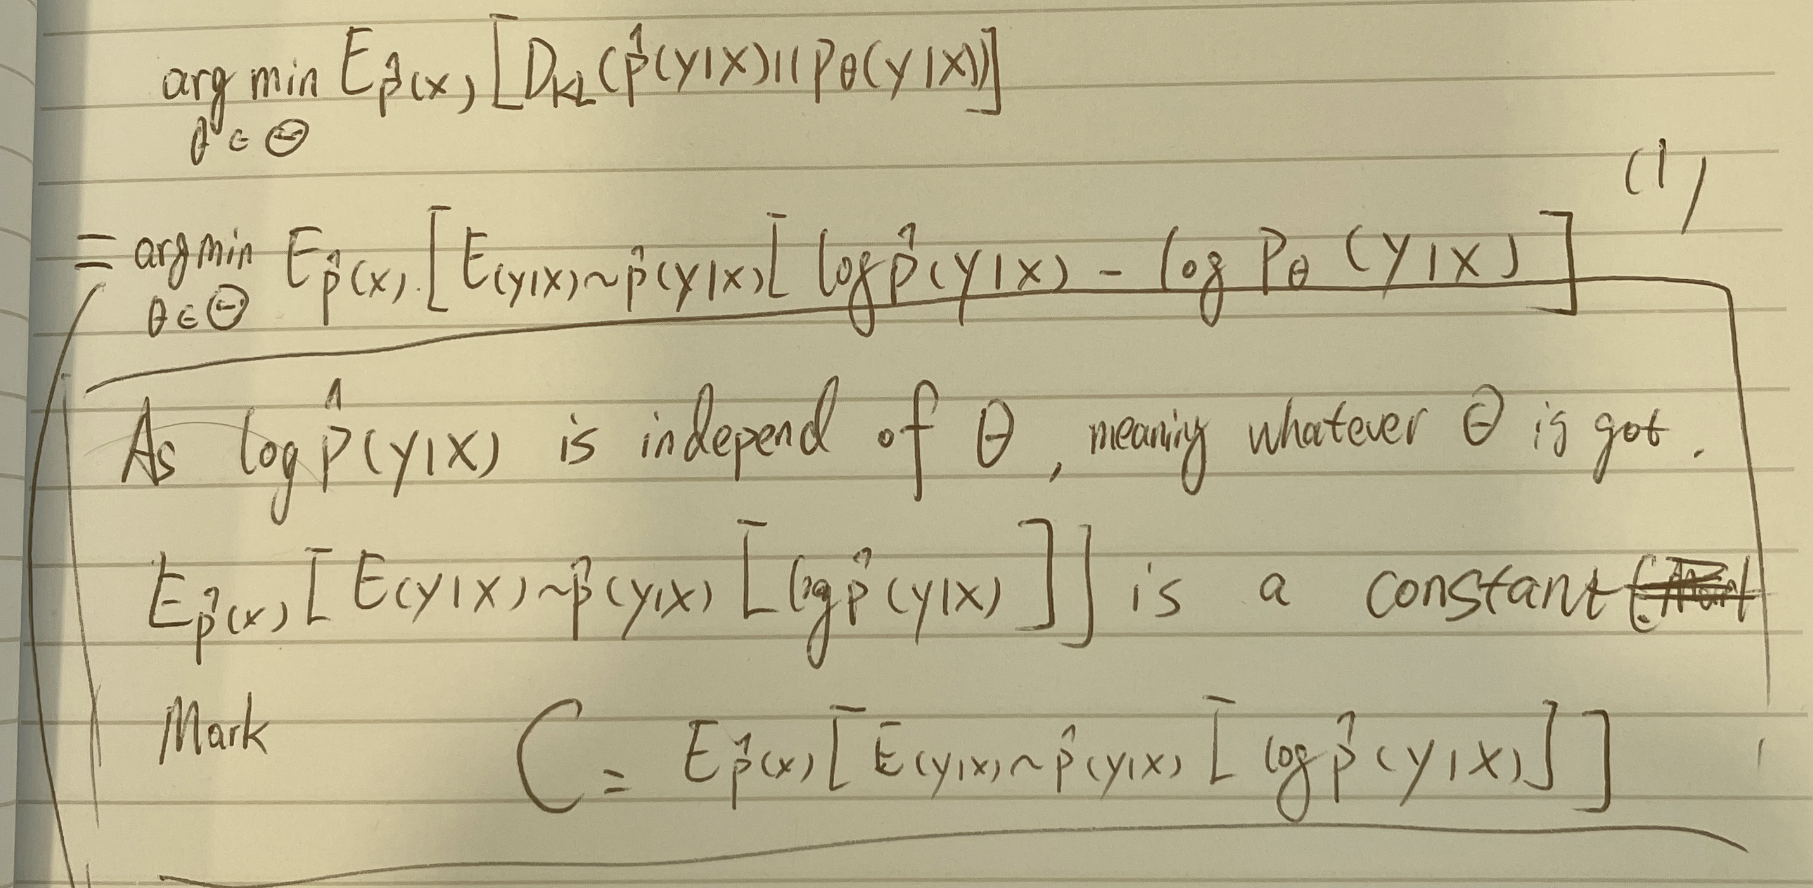
\includegraphics[width=0.8\linewidth]{PS1-1-1.png}
    
    Then use constant \(C\) to replace the first part in the equation: \\
    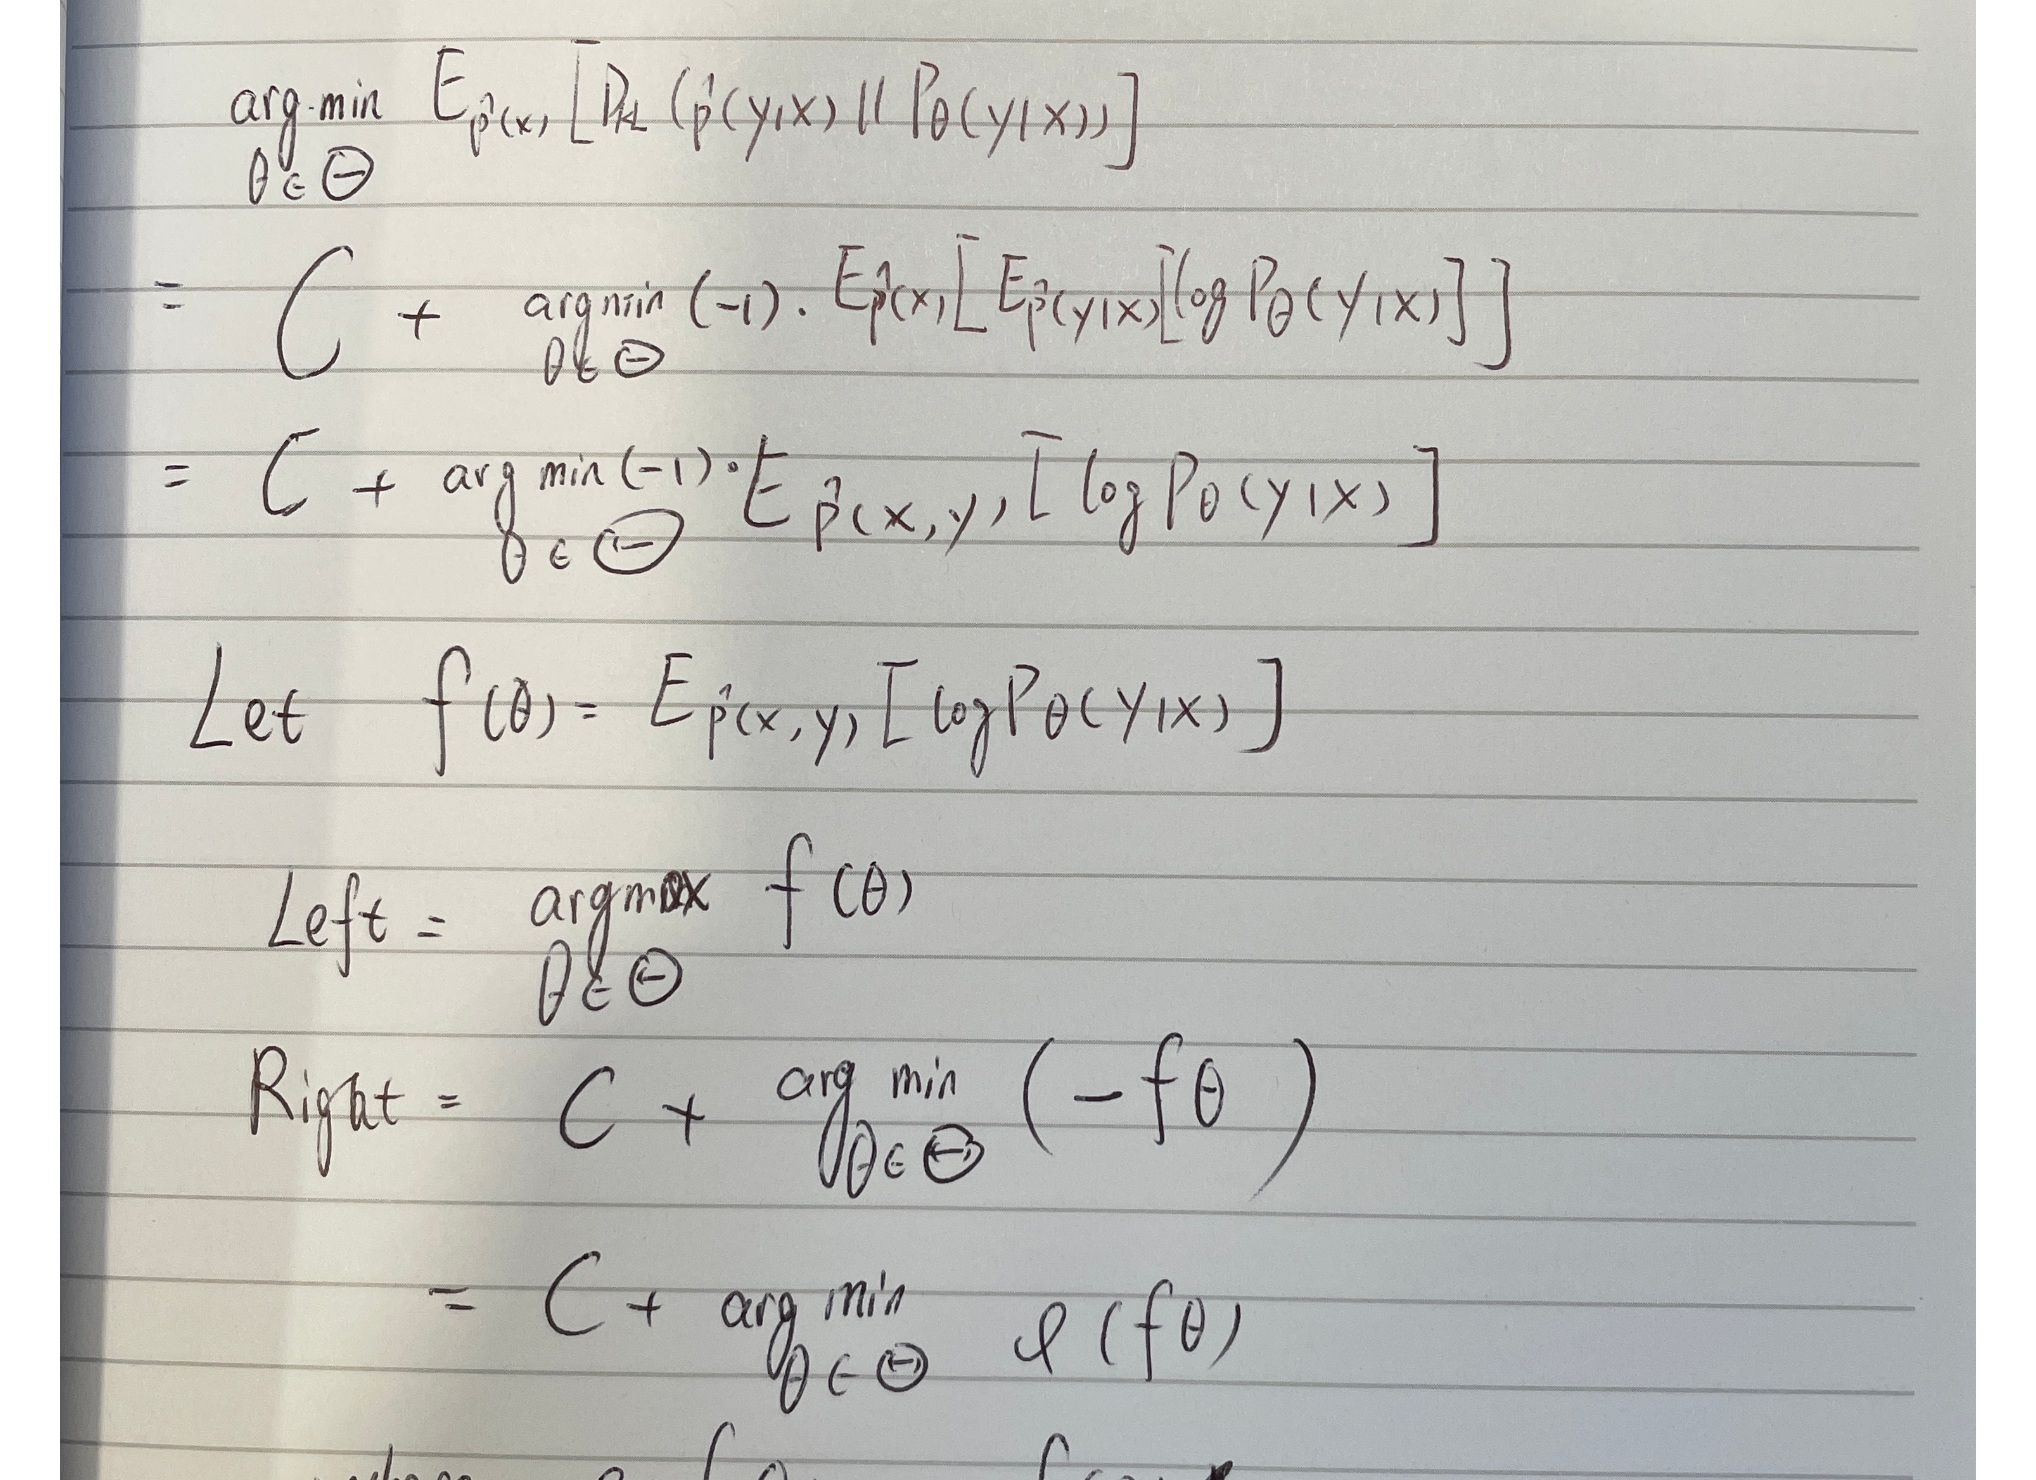
\includegraphics[width=0.8\linewidth]{PS1-1-2.png}
    
    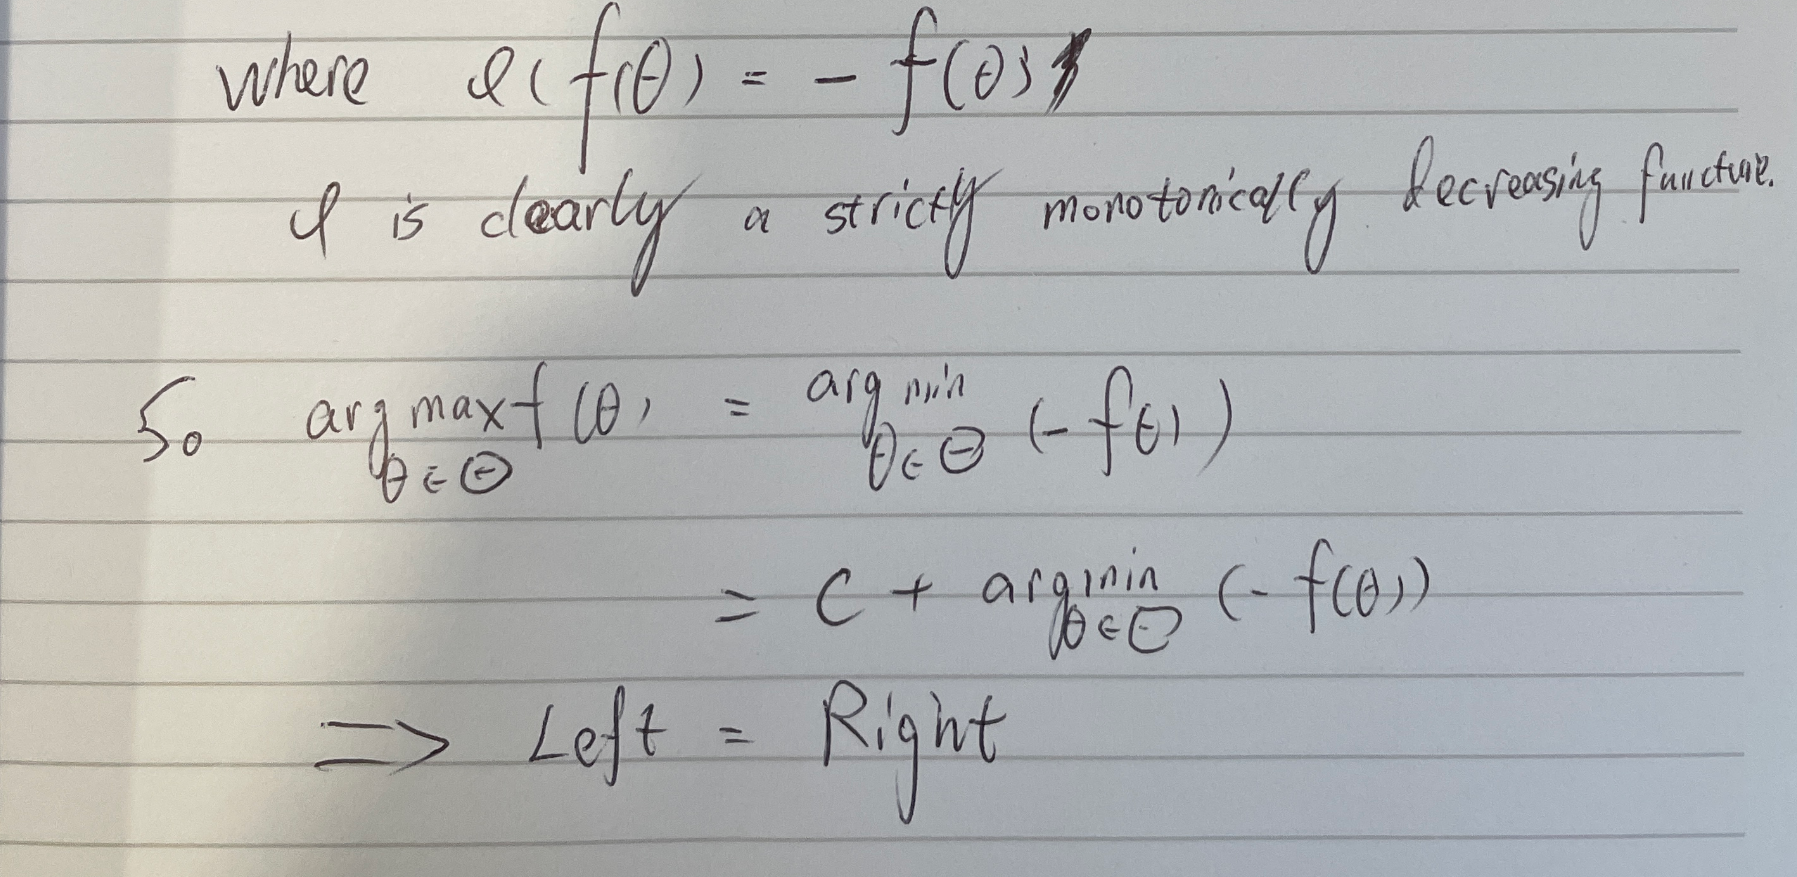
\includegraphics[width=0.8\linewidth]{PS1-1-3.png}
    
    

    % ### END CODE HERE ###
\end{answer}
% <SCPD_SUBMISSION_TAG>_1

\clearpage

\LARGE
2
\normalsize
% <SCPD_SUBMISSION_TAG>_2
\begin{answer}
    To help you get start consider that:

    \begin{center}
        $p_{\theta}(y \mid x) = \frac{p_{\theta}(x,y)}{p_{\theta}(x)}$
        $= \frac{\pi_{y} \cdot \exp\left(- \frac{1}{2\sigma^2} \left(x-\mu_{y}\right)^{\top}\left(x-\mu_{y}\right)\right) \cdot Z^{-1}(\sigma)}{\sum_{i} \pi_i \cdot \exp\left(- \frac{1}{2\sigma^2}\left(x-\mu_{i}\right)^{\top}\left(x-\mu_{i}\right)\right) \cdot Z^{-1}(\sigma)}$
    \end{center}

    where $Z(\sigma)$ is the Gaussian partition function (which is a function of $\sigma$). 
    
    % ### START CODE HERE ###
    % From Bayes' Rule: 
    % \begin{equation}
    %     p_{\theta}(y \mid x) = \frac{p_{\theta}(x,y)}{p_{\theta}(x)} = \frac{p_{\theta}(x \mid y) p_{\theta}(y)}{p_{\theta}(x)}
    % \end{equation}

    % Note that:
    % \begin{equation}
    %     p_{\theta}(x \mid y) = N(x \mid \mu_y, \sigma^2I) \textbf{ and }
    %     p_{\theta}(y) = \pi_y
    % \end{equation}

    % Then Gaussian Mixture Components:
    % \begin{equation}
    %     p_{\theta}(y \mid x) = \frac{N(x \mid \mu_y, \sigma^2I) \pi_y}{p_{\theta}(x)} 
    % \end{equation}

    % Thus:
    % \begin{equation}
    %     p_{\theta}(x) = \sum_{i=1}^{k} N(x \mid \mu_i, \sigma^2I) \pi_i
    % \end{equation}

    % From equation (3), perform log on both sides and get:
    % \begin{equation}
    %     \log p_{\theta}(y \mid x) = \log N(x \mid \mu_y, \sigma^2I) + \log \pi_y - \log p_{\theta}(x)
    % \end{equation}

    % Then:
    % \begin{equation}
    %     \log p_{\theta}(y \mid x) = -\frac{n}{2}\log(2\pi) - \frac{1}{2}\log \mid \sigma^2 I \mid - \frac{1}{2\sigma^2}(x - \mu_y)^T(x - \mu_y) + \log \pi_y - \log p_{\theta}(x)
    % \end{equation}

    % Then:
    % \begin{equation}
    %     \log p_{\gamma}(y \mid x) = x^T w_y + b_y - \log \sum_{i=1}^{k} \exp(x^T w_i + b_i)
    % \end{equation}

    % Thus we can pick:
    % \begin{equation}
    %     w_y = (1/\sigma^2) \mu_y
    % \end{equation}

    % \begin{equation}
    %     b_y = \log \pi_y - (1/2\sigma^2) \mu_y^T \mu_y - (n/2) \log(2\pi) - (1/2) \log \mid \sigma^2I \mid
    % \end{equation}


    From the above equation, take log on both sides:
    \begin{equation}
         \log p_{\theta}(y \mid x) = - \frac{1}{2\sigma^2}(x - \mu_y)^T(x - \mu_y) + \log \pi_y - \log p_{\theta}(x) - log(\sum_{i} \pi_i \cdot \exp\left(- \frac{1}{2\sigma^2}\left(x-\mu_{i}\right)^{\top}\left(x-\mu_{i}\right)\right) \cdot Z^{-1}(\sigma))
    \end{equation}

    
    \begin{equation}
         \log p_{\theta}(y \mid x) = \frac{1}{\sigma^2}x^T\mu_y - \frac{1}{2\sigma^2}x^Tx - \frac{1}{2\sigma^2}\mu_y^T\mu_y + \log \pi_y - \log p_{\theta}(x) - log(\sum_{i} \pi_i \cdot \exp\left(- \frac{1}{2\sigma^2}\left(x-\mu_{i}\right)^{\top}\left(x-\mu_{i}\right)\right) \cdot Z^{-1}(\sigma))
    \end{equation}

    From the question:
    \begin{equation}
        p_\gamma(y \mid x) = \frac{exp(x^T w_y + b_y)}{\sum_{i=1}^{k}(exp(x^T w_i + b_i))} \\
    \end{equation}

    From (3) take log on both sides:
    \begin{equation}
        log p_\gamma(y \mid x) = x^T w_y + b_y - log(\sum_{i=1}^{k}(exp(x^T w_i + b_i)))
    \end{equation}

    The question is asking to find \(w_y\) and \(b_y\) that makes question (2) equations equation (4).

    Then
    \begin{equation}
        w_y = \frac{1}{\sigma^2}\mu_y
    \end{equation}
    \begin{equation}
        b_y = \log \pi_y - \frac{1}{2\sigma^2} \mu_y^T \mu_y - (1/2) \log \mid \sigma^2I \mid
    \end{equation}

    % ### END CODE HERE ###
\end{answer}
% <SCPD_SUBMISSION_TAG>_2


\clearpage

\LARGE
3a
\normalsize

% <SCPD_SUBMISSION_TAG>_3a
\begin{answer}
    % ### START CODE HERE ###
    \((X_1, X_2, ..., X_n)\) can be fully represented by a table where each cell corresponds to a unique combination of outcomes for all the variables. Total number of cells is:

    \begin{equation}
        k_1 * k_2 * ... * k_n = \prod_{i=1}^{n}k_i
    \end{equation}

    However, since the probabilities in a distribution must sum to 1, so the total number of independent parameters is

    \begin{equation}
        \prod_{i=1}^{n}k_i - 1
    \end{equation}
    % ### END CODE HERE ###
\end{answer}
% <SCPD_SUBMISSION_TAG>_3a

\LARGE
3b
\normalsize

% <SCPD_SUBMISSION_TAG>_3b
\begin{answer}
    % ### START CODE HERE ###
    If variables \((X_1, X_2, ..., X_n)\) are mutually independent, then there are  \(\sum_{i=1}^{n}(k_i - 1)\) total number of independent parameters.
    % ### END CODE HERE ###
\end{answer}
% <SCPD_SUBMISSION_TAG>_3b

\LARGE
3c
\normalsize

% <SCPD_SUBMISSION_TAG>_3c
\begin{answer}
    % ### START CODE HERE ###
    For each \(i > m\) and \(i <= n\), it requires

    \begin{equation}
      k_i * k_{i-1} * ... * k_{i-m} - 1 = \prod_{j=i-m}^{i}k_i - 1
    \end{equation}

    For each \(i <= m\), it requires

    \begin{equation}
        k_i - 1
    \end{equation}

    Combine (9) and (10) together, total number of parameters are:

    \begin{equation}
        \sum_{j=1}^{m}(k_j-1) + \sum_{j=m+1}^n(\prod_{j=i-m}^{i}k_i - 1)
    \end{equation}
    % ### END CODE HERE ###
\end{answer}
% <SCPD_SUBMISSION_TAG>_3c

\clearpage

\LARGE
4
\normalsize

% <SCPD_SUBMISSION_TAG>_4
\begin{answer}
    To provide more direction consider proving (*) or (**) below:
    Consider the simple case of describing a joint distribution over $(X_1,X_2)$ using 
    the forward versus reverse factorizations. Consider the forward factorization where

    \begin{center}
        $p_f(x_1) = \calN(x_1 \mid 0,1)$ \\
        $p_f(x_2 \mid x_1) = \calN(x_2 \mid \mu_2(x_1), \epsilon)$
    \end{center}

    for which

    \begin{center}
        $
        \mu_2(x_1) = 
        \begin{cases}
            0 & \text{if } x_1 \le 0 \\
            1 & \text{otherwise}
        \end{cases}
        $
    \end{center}

    (*) This construction makes $p_f(x_2)$ a mixture of two distinct Gaussians, which $p_r(x_2)$ cannot match, since $p_f(x_2)$ is 
    strictly Gaussian. Any counterexample of this form, which makes $p_f(x_2)$ non-Gaussian, suffices for full-credit.

    (**) Interestingly, we can also intuit about the distribution $p_f(x_1 \mid x_2)$. If one chooses a very small positive $\epsilon$, then the 
    corresponding $p_f(x_1 \mid x_2)$ will approach a truncated Gaussian distribution, which cannot be approximated by the Gaussian $p_r(x_1 \mid x_2)$
    \footnote{This observation will be useful when we move on to variational autoencoders $p(z,x)$ (where $z$ is a latent variable) and discuss the 
    importance of having good variational approximations of the true posterior $p(z \mid x)$}.

    Optionally, we can prove (*) and a variant of (**) which states that, any $\epsilon > 0$, the distribution:

    \begin{center}
        $p_f(x_1 \mid x_2) = \frac{p_f(x_1,x_2)}{p_f{x_2}}$
    \end{center}

    is a mixture of truncated Gaussians whose mixture weights depend on $\epsilon$.

    % ### START CODE HERE ###
    \textbf{Answer: No}
    
    \textbf{Counterexample (n=2)}:
    
    Let's consider a simple case with two variables, (\(X_1\)) and (\(X_2\)), as suggested in the hint.
    
    Define the forward model as follows:
    \begin{equation}
        (p_f(x_1) = \mathcal{N}(x_1 \mid 0, 1))
    \end{equation}

    \begin{equation}
    \begin{split}
        (p_f(x_2 \mid x_1) = \mathcal{N}(x_2 \mid \mu_2(x_1), \epsilon)) \textbf{ where:} \\
        \mu_2(x_1) = \begin{cases} 
                   0 & \text{if } x_1 \le 0 \\
                   1 & \text{otherwise}
               \end{cases}
    \end{split}
    \end{equation}

    Given that:
    \begin{equation}
        p_f(x_1, x_2) = p_f(x_1) * p_f(x_2 \mid x_1)
    \end{equation}

    This construction makes \(p_f(x_2)\) a mixture of two distinct Gaussians.

    For the reverse:
    \begin{equation}
        p_r(x_1, x_2) = p_r(x_2) * p_r(x_1 \mid x_2)
    \end{equation}

    For \(p_r(x_2)\) to match the behavior of \(p_f(x_2)\) as described above, it needs to be a mixture of two distinct Gaussians, which can't be achieved if we model \(p_f(x_2)\) directly.
    % ### END CODE HERE ###
\end{answer}
% <SCPD_SUBMISSION_TAG>_4

\clearpage

\LARGE
5a
\normalsize

% <SCPD_SUBMISSION_TAG>_5a
\begin{answer}
    % ### START CODE HERE ###
    \begin{equation}
    \begin{split}
        E[A] & = E[\frac{1}{k} * \sum_{i=1}^{k} p(x \mid z^{(i)})] \\
             & = \frac{1}{k} * \sum_{i=1}^{k}E[p(x \mid z^{(i)})] \\
             & \sim \frac{1}{k} * \sum_{i=1}^{k} \int_x p(x \mid z)p(z)dz \textbf{ since } z^{(i)} \sim p(z)\\
             & = \int_x p(x \mid z)p(z) dz \\
             & = \int_x p(x, z) dz \\
             & = p(x)
    \end{split}
    \end{equation}
    % ### END CODE HERE ###
\end{answer}
% <SCPD_SUBMISSION_TAG>_5a

\LARGE
5b
\normalsize

% <SCPD_SUBMISSION_TAG>_5b
\begin{answer}
    % ### START CODE HERE ###
    \(log\) is a concave function, and thus by Jensen's inequality:

    \begin{equation}
        E[log(A)] <= log(E[A])
    \end{equation}

    From question 5a, we know that \(E(A)=p(x)\), thus:
    \begin{equation}
        E[log(A)] <= log(p(x))
    \end{equation}

    This means \(log(A)\) is a \textbf{biased} estimator.
    % ### END CODE HERE ###
\end{answer}
% <SCPD_SUBMISSION_TAG>_5b

\clearpage

\LARGE
6a
\normalsize

% <SCPD_SUBMISSION_TAG>_6a
\begin{answer}
    % ### START CODE HERE ###
    Each \(a_i\) has \(2\) possible values, and thus we need to find the minimum integer \(n\) that:

    \begin{equation}
        2^n >= 502457
    \end{equation}

    Then
    \begin{equation}
        n >= log_2 50257 = 15.617
    \end{equation}

    Thus the minimum possible integer \(n\) is \(16\).
    % ### END CODE HERE ###
\end{answer}
% <SCPD_SUBMISSION_TAG>_6a

\LARGE
6b
\normalsize

% <SCPD_SUBMISSION_TAG>_6b
\begin{answer}
    % ### START CODE HERE ###
    In the embedding layer, total parameter is (total possible tokens) * (vector dim). Thus the increase in the embedding layer is:

    \begin{equation}
        (60000-50257)*768=7482624
    \end{equation}

    The the number of the parameters in the GPT-2 module is not changed.

    In the Fully-Connected Layer, input is 768 dim, output is from 50257 dim to 60000. So the parameter increase is:

    \begin{equation}
        (60000-50257)*768=7482624
    \end{equation}

    Add all of them together, the total parameter increase is:
    \begin{equation}
        7482624 + 7482624 = 14965248
    \end{equation}
    % ### END CODE HERE ###
\end{answer}
% <SCPD_SUBMISSION_TAG>_6b

\LARGE
6g
\normalsize

% <SCPD_SUBMISSION_TAG>_6g
\begin{answer}
    % ### START CODE HERE ###
    % ### END CODE HERE ###
\end{answer}
% <SCPD_SUBMISSION_TAG>_6g

% <SCPD_SUBMISSION_TAG>_entire_submission

\end{document}